\section{Data handling}
\label{sec:datahandling}

\begin{figure}[H]
    \centering
    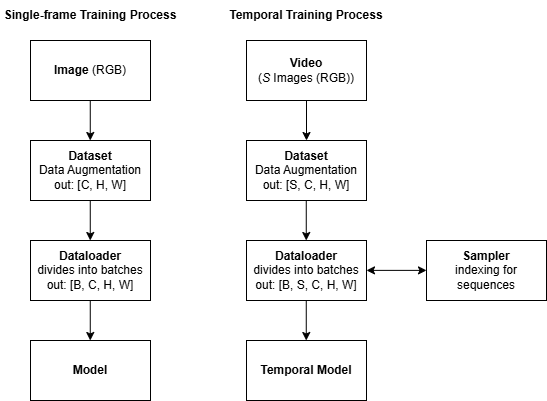
\includegraphics[width=0.6\linewidth]{PICs/temporalModels/Datahandling.png}
    \caption{Comparison between data handling processes for single-frame training and the proposed temporal training.}
    \label{fig:dataHandlingProcess}
\end{figure}

The Dataset class reads in images according to an index, performs online data augmentation and outputs a tensor.
The Dataloader iterates through the dataset step by step and calls the dataset class using the indices.
It can either move step by step or rely on a sampler to dictate the stepping pattern.
In temporal training, a sampler is essential to manage sequences, avoiding out-of-bound errors and preventing scene intermixing.
Furthermore the Datalaoder creates batches and therefore adds the dimension $B$ to the tensor.

The training consists of a pre-defined number of epochs, which presents one training cycle.
In each epoch, the Dataloader is used to feed the model one batch.
Then the model predicts, calculates the loss according to this prediction and performs the back propagation to optimize the model.
In the same cycle the validation is done, in which the Dataloader feeds the model samples of the validation set.
Here only the prediction is done and the loss is calculated.
Two additional steps are done in an epoch after training and validating.
On the one hand, the scheduler updates the learning rate.
In this work the OneCycleLR scheduler \cite{pytorch_oneCycleLR_docu} is used, which calculates the used learning rate according to a formula.
On the other hand, when the validation loss reaches a new minimum, the model is saved.
This way the model with the lowest loss is obtained at the end of all epochs.